\documentclass[twocolumn]{article}
\usepackage{graphicx}  % For including images
\usepackage{amsmath}   % For advanced math symbols
\usepackage{url}       % For clickable URLs
\usepackage{xcolor}
\usepackage{geometry}   
\usepackage{hyperref}% To reduce margins
%\setlength{\droptitle}{-2cm} % Reduce space before the title
\usepackage[utf8]{inputenc}
\usepackage{soul} % Pacote para highlight
\usepackage{xcolor}
\sethlcolor{lightgray}


% Adjusting margins
\geometry{
    left=1.5cm,
    right=1.5cm,
    top=1cm,
    bottom=2cm,
    columnsep=1cm % Spacing between columns
}

\title{LN - Project Report}

\author{
    Group 31 \\[1ex] % Adjust spacing if needed
    \\
    Salvador Florêncio — ist1102706, Tiago Silva — ist1103811, Luís Calado — ist1103883 \\
}
\date{}

\begin{document}

\maketitle

\section{Models}
In our initial approach, we applied a Multinomial Naive Bayes classifier to the dataset preprocessed using the Term Frequency-Inverse Document Frequency (TF-IDF) method, based on the notebook provided in lab classes and an approach to a similar challenge found on \href{https://www.kaggle.com/code/imgowthamg/movie-genre-classification}{Kaggle}. By doing so, we were able to achieve an accuracy score of 37\%. Then, by using the CountVectorizer method instead of TF-IDF, we achieved an accuracy of 64\%. 
%However, despite its good performance, Naive Bayes works on the assumption that input words are independent, and, as such, could fail to represent the complexity of the classification classes.

%Incluir isto: One problem with Naive Bayes is that the bag-of-word feature as well as the conditional independence assumption are not realistic and may not capture the meaning of sentences in text.

Building on this, we explored various models, including a Support Vector Machine with a TF-IDF vectorizer, Logistic Regression, Random Forests and even experimented a deep learning model, TinyBERT \cite{tinybert}, in an effort to achieve higher accuracy. 
\vspace{-0.6 cm}
\subsection*{Feature-based models}
\vspace{-0.2 cm}
Our best feature-based model was the Support Vector Machine with a linear kernel combined with TF-IDF Vectorizer, resulting in an accuracy of 69\%, while our second-best model was Logistic Regression, also combined with TF-IDF Vectorizer (68\% accuracy).

For \textbf{pre-processing}, we tried various approaches, with our best one being: lowercasing; removing punctuation, stopwords, URLs (we noticed one of the plots contains a URL), and removing actor names, as we observed that in many plots, actor names appeared alongside character names (e.g., "Charley Kittridge (Joe Dorsey)"). \hspace{-0.1cm}We also tokenized the text and used lemmatization. \hspace{-0.08cm}Stemming yielded worse results, so we discarded it.
%[The evaluation results for the SVM model fine-tuned with the given dataset are shown in figure \ref{fig:conf} and table \ref{tab:my_table}. The overall accuracy was 69\%, which is on par with the current state of the art for this task. ]
\vspace{-0.6 cm}
\subsection*{Sequence models}
\vspace{-0.2cm}
To explore sequence models, we employed TinyBERT \cite{tinybert}, a BERT \cite{bertpaper} flavour with fewer parameters that retains the ability to learn the rich knowledge embedded in the pre-trained BERT model. The specific variant we used is \href{https://huggingface.co/huawei-noah/TinyBERT_General_4L_312D}{\texttt{TinyBERT\_General\_4L\_312D}}, available through Hugging Face’s \texttt{transformers} library. 
The model was fine-tuned for the task by setting up a custom PyTorch \texttt{Dataset} and using the \texttt{AutoTokenizer} to tokenize the input data. However, this transfer learning technique did not yield an improvement in accuracy (67.7\%) compared to our previous models, leading us to select the \underline{SVM with TF-IDF model} as our best-performing model.

\section{Experimental Setup and Results}
\subsection*{Support Vector Machine with TF-IDF}
We applied a manual 90-10 test split and trained the model using 10-fold cross-validation on the training set. %, keeping an eye on the relationship between the score on the test and validation sets, and tuning the hyperparameters accordingly. 
For the tuning of the hyperparameters, we also used \texttt{GridSearchCV} together with a pipeline to find the best combination of parameters for \texttt{TfidfVectorizer} and SVM. However, since \texttt{GridSearchCV} exhaustively searches all possible parameter combinations, it took a significant amount of time to run. As a result, we opted for \texttt{RandomizedSearchCV}, which explores only a fixed number of hyperparameter combinations. %Along with some manual tuning, this approach helped us to optimize the model’s performance more efficiently.

For the SVM parameters, we used bigrams to capture word relationships and set \texttt{max\_features=20000} to filter out the least relevant terms, reducing the risk of overfitting. Additionally, we enabled \texttt{sublinear\_tf%=True
}, as it provided better results \cite{fei2019movie}.

We opted for the linear kernel as it provided the best accuracy in our experiments, though the sigmoid kernel also yielded good results. However, the sigmoid kernel is typically suited to datasets with a sigmoidal shape, and requires careful fine-tuning to find generalizable decision boundaries. Due to its more specific use cases, the sigmoid kernel is less commonly used, which led us to favor the linear kernel for this task.

%\vspace{-0.6 cm}
\subsection*{TinyBERT}
%\vspace{-0.4 cm}

An 85-15 train-test split was used to evaluate the model's performance. %This setup allowed us to tune the hyperparameters by comparing the results on both the validation and test sets, optimizing the model based on these evaluations.
The training loop was structured using mixed precision for performance gains, with \texttt{GradScaler} handling floating point operations. We optimized the model using AdamW optimizer, with learning rates of \{3e-5, 5e-5, 1e-4\}. The model was trained for \{3, 4\} epochs with a batch size of \{16, 32\}, using cross-entropy loss as the loss function. During each epoch, we truncated the input sequences to TinyBERT's maximum token limit of 512 (see  \nameref{sec:discussion}) and ran forward and backward passes to calculate the loss and update the model weights accordingly.

For evaluation, we transitioned the model to evaluation mode and computed the accuracy on the validation set. This fine-tuning approach allowed us to achieve an accuracy no higher than 67.7\%.

\subsection*{Results}
\vspace{-0.2cm} 
From the recall scores for each label, it is clear that they are quite inconsistent. For instance, the recall for the "Western" genre is 0.91, while for "Sci-Fi" genre it is only 0.40. This gap is primarily due to the challenging nature of the task, even for human annotators, and also because of the fact that the dataset is unbalanced (\href{https://ibb.co/s1p8PMQ}{genre distribution}\footnote{See dataset genre distribution; limited space required this link.}). The precision ranges from 0.55, for "Drama", up to 0.95, for "Western".
\vspace{-0.3cm}
\begin{figure}[!ht]
    \centering
    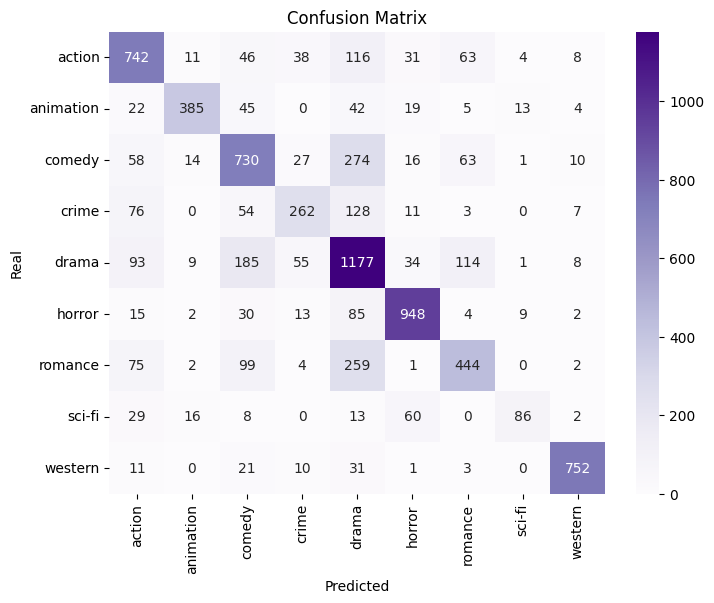
\includegraphics[width=0.45\textwidth]{confusion-matrix.png} % Replace with actual image path
    \caption{Confusion matrix with SVM with TF-IDF}
    \label{fig:conf}
\end{figure}
\vspace{-0.6cm}
\begin{table}[!ht]
\centering
\caption{Evaluation metrics with SVM with TF-IDF}
\label{tab:my_table}
\vspace{0.2cm}
\resizebox{0.4\textwidth}{!}{ % Reduced to 0.4 from 0.5
\begin{tabular}{|c|c|c|c|c|}
\hline
 \textbf{Label} & \textbf{Precision} & \textbf{Recall} & \textbf{F1-Score} & \textbf{Support} \\
\hline
\texttt{Action} & 0.66 & 0.70 & 0.68 & 1059 \\
\texttt{Animation} & 0.88 & 0.72 & 0.79 & 535 \\
\texttt{Comedy} & 0.60 & 0.61 & 0.61 & 1193 \\
\texttt{Crime} & 0.64 & 0.48 & 0.55 & 541 \\
\texttt{Drama} & 0.55 & 0.70 & 0.62 & 1676 \\
\texttt{Horror} & 0.85 & 0.86 & 0.85 & 1108 \\
\texttt{Romance} & 0.64 & 0.50 & 0.56 & 886 \\ 
\texttt{Sci-fi} & 0.75 & 0.40 & 0.52 & 214 \\ 
\texttt{Western} & 0.95 & 0.91 & 0.93 & 829 \\ 
\hline
\end{tabular}%
}
\end{table}
\vspace{-0.4cm}
\section{Discussion}
\label{sec:discussion}
\vspace{-0.2cm}
Right from the beginning, we recognized that predicting movie genres (with 9 labels...) from the plot would be a challenging endeavor, even for a human classifier. 

On one hand, some movie plots were very short (\href{https://ibb.co/JQfxGBx}{word counts in plot descriptions} \footnote{See word counts in plot descriptions; limited space required this link.}), which made it even more difficult for our model to accurately predict their genre. On the other hand, a significant number of movie plots exceeded 512 words and were truncated by TinyBERT, as the model only accepts up to 512 tokens.
 

The research was limited to only movies from the given \texttt{train.txt} dataset consisting of 8041 movies, a far lower number than the \href{https://www.kaggle.com/datasets/jrobischon/wikipedia-movie-plots}{entire dataset at Kaggle} which exceeds 134 000 plots. If the dataset was not restricted, then there would likely have been an increase in accuracy.

 A careful look at the confusion matrix reveals
that mislabeling took place mostly across drama/comedy lines. This task might be difficult even for human classifiers, we present some examples:

\hl{\texttt{Plot: (...) One day, he receives a surprise assignment: to fly over 12,000 kilometers of enemy waters to protect a girl named Juana del Moral. This mission is actually a covert operation as the original escort was taken down by the enemy. (...)}}

\texttt{Ground-truth}: animation | \texttt{Predicted}: action

It is very challenging to know whether a movie is animated only by looking at its plot.

\hl{\texttt{Plot: A mother and wife stricken with memory loss allows a dysfunctional family a second chance at harmony and happiness}}

\texttt{Ground-truth}: comedy | \texttt{Predicted}: drama

Differentiating between comedy and drama can be incredibly difficult, since drama can be used as a source of comedy.

\hl{\texttt{Plot: Satyameva Jayate is the story of a traffic constable who witnesses a murder committed by a politician’s son in day light and the reactions he had to face when he tries to bring the culprits to book. As a bunch of dishonest bureaucrats and corrupted cops acts against him, he had to turn into the long-haired, local goon Pandiya to take revenge.}}

\texttt{Ground-truth}: romance | \texttt{Predicted}: action

This movie is a romance, but there is no hint of it in the plot synopsis.

%The performance of our model seems to be in line with what we identified. The difficulty of the domain was evident - no matter the models we tried, or the pre-processing we did, we never seemed to get scores well above 90\%. 

\hl{\texttt{Plot: A happily married couple's life is turned upside down when they are approached by a woman also claiming to be the husband's wife.}}

\texttt{Ground-truth}: romance | \texttt{Predicted}: drama

Many romance movie synopses can be interpreted as being drama and vice-versa, since movies are very often both.

\hl{\texttt{Plot: A respectable woman's position in society is threatened by a blackmailer.}}

\texttt{Ground-truth}: drama | \texttt{Predicted}: crime

Some plot synopses are incredibly short and can be interpreted as being part of a multitude of genres.


\vspace{-0.3cm}
\section{Future Work}
\vspace{-0.3cm}
If given more time, we plan to address the class imbalance in our dataset by creating custom datasets that give more weight to labels with fewer examples, while reducing the influence of those that are more frequent. We also aim to explore data augmentation techniques to achieve a more balanced dataset.

There is a potential in further tuning our TinyBERT model. Although it came close to being our best model, with improved fine-tuning, we believe it could yield even better results. One possible approach would be to freeze some of the initial layers and then train the entire architecture \cite{zhao2022methods}. 

Another area of interest is the fact that movies often belong to multiple genres. So we would like to explore strategies for addressing cases where a movie has more than one genre label.
\newpage
\small
\bibliographystyle{plain}
\bibliography{refs}

\end{document}


